\chapter{Agents}
In this chapter the different agents are introduced and discussed.

\section*{Simplifications}
To limit the scope of the project and to be able to concentrate on the 'card play' aspect of Tichu, I decided to simplify the agents as follows:
\begin{description}
    \item[No Trading] The agents all trade random cards. This has the same effect as omitting the trading phase. % TODO This phase is astonishingly complicated to do good and deserves a project for itself. more, influenced by cooperative, tichu, planing, overall strategy
    \item[No Tichu announcement] As mentioned in section~\ref{sec:tactics}, points won with Tichus often dominate points won by wining tricks. This diverts from the 'card play' aspect. Therefore all Agents are implemented such that they never announce any Tichu. % TODO and thus only win by playing better than the opponent. As another consequence, the importance of cooperative play is reduced. % TODO write nicer
    \item[Bombs not anytime] For simplicity and ease of simulation, a player can only play when it's his turn. That means bombs can not be played out of turn. This does not have a big impact on the game play overall, since it is rare to gain an advantage in playing a bomb out of turn.
    % TODO  As a result the agents can't learn strategies involving bluffing or 'laying traps' (for example waiting for the Dragon, then bomb it to gain points. or bomb a combination that otherwise can't be beaten.)... would increase branching factor and would slow down mcts considerably. could be made efficient but was too complicated.
    %\item[No Wish] For a similar reason as the 'no Tichu' simplification, the agents do not wish any card.
    \item[Random Wish] There are different strategies to determine which cards to wish. To not introduce domain knowledge, all agents wish for a random card.
\end{description}

\section{Background}
\label{sec:background}
This section contains a short overview of the main algorithms used by the different agents.

An important notion is the \textbf{gametree}, which is a tree containing as nodes all possible gamestates and as edges the (game)actions leading from a parent state to a child state. The root is the initial state of the game, and the leafs are states in which the game ended (one player or team has won).

\subsection{Minimax Search}
Given a gametree, the optimal strategy can be determined from the minimax value of each node. This value denotes how 'good' a gamestate is for the searching player and is computed as follows:
$$
    minimaxval(s)=
\begin{cases}
    Reward(s), & \text{if s is terminal} \\
    \max_{a\in Actions(s)} minimaxval(next(s, a)), & \text{if player(s) = searching player} \\
    \min_{a\in Actions(s)} minimaxval(next(s, a)), & \text{otherwise}
\end{cases}
$$
where $s$ is a gamestate, $Reward(s)$ denotes the reward for the searching player in $s$, $Actions(s)$ is the set of legal actions in $s$, $player(s)$ denotes the player able to play in $s$ and $next(s, a)$ is the resulting state when playing action $a$ in $s$. \newline
This algorithm performs a complete depth-first search of the gametree, which is computationally unfeasible in most games, but it is a good theoretical baseline for other algorithms.

Despite this, it is possible to use minimax in larger games by stopping at non terminal states and evaluating them with an $utility$ function.
Minimax has been successfully used in games where it is possible to create a good $utility$ function, most prominently in chess.

Furthermore, it is possible to prune away large parts of the searchtree without loosing accuracy using \textbf{alpha-beta pruning}. This method makes use of the fact that some subtrees don't influence the final result since the players never play suboptimal actions. For more details see \cite[chapter 5, p.~170+]{russel14} or any textbook about artificial intelligence.

\subsection{Monte Carlo Tree Search (MCTS)}
Similar to minimax search, MCTS also searches the gametree, but uses simulated games to evaluate nonterminal states and thus does not need an utility function. This is especially useful for games where it is hard to determine whether a state is 'good' or 'bad' for a player, for example in games with hidden information, but also in perfect information games such as GO.

The algorithm iteratively builds a subtree of the gametree where the root corresponds to the current state of the game. Each iteration consists of the 4 phases shown in Fig.~\ref{fig:mcts_phases}:
\newline\textbf{Tree Selection} The algorithm traverses the (in previous iterations built up) gametree until it reaches a leaf-node. The decision which actions to follow during the traversal is determined by the \textit{tree policy}. The tree policy attempts to balance considerations of exploration (look in areas that have not been well sampled yet) and exploitation (look in areas which appear to be promising).
An often used tree policy is the UCT (Upper Confidence bound for Trees) formula proposed by \cite{uct} (see section \ref{sec:uct}).
\newline\textbf{Expansion} Once arrived at a leaf state, one more action is chosen and a node for the resulting gamestate is added to the tree. Form this state a \textit{simulation} (or \textit{rollout}) is performed.
\newline\textbf{Simulation} A simulation is the run from a gamestate to a terminal state of the game. During simulation the moves are made according to the \textit{default policy}, which typically chooses an action uniformly at random.
\newline\textbf{Backpropagation} The final state is evaluated and the reward for each player is calculated. The reward is then used to update the statistics of the nodes visited during tree selection, which in turn is used for the \textit{tree policy} in future iterations.

The search can be terminated at any point which makes MCTS especially suitable for games with time or computational resource constraints.

\begin{figure}[h]
    \begin{center}
      \includegraphics[width=0.58\textwidth]{images/basic_mcts_process.png}
      \caption[Basic MCTS process]
      {The basic steps of MCTS. Source \cite{perez13}}
      \label{fig:mcts_phases}
    \end{center}
\end{figure}


\subsection{Determinization and Perfect Information MCTS (PIMCTS)}
\textbf{Determinization} is the process of taking a gamestate with hidden information and creating ('determining') a perfect information state that is consistent with the hidden information. In essence, determinization chooses one out of the many possible perfect information gamestates for a given hidden information gamestate.

To deal with hidden information, PIMCTS performs several instances of MCTS, each on a different determinization. The best action is then chosen based on the results of the individual MCTS.
This approach was successfully used for the game Bridge in \cite{bridge}, but has two main drawbacks, also described in \cite{bridge} and further explored in \cite{pimcts} and \cite{ismcts}:
\newline\textbf{Strategy fusion:} An agent can only make one decision in each hidden information state, but in different determinizations different decisions can be made based on the perfect information. This lets the agent 'believe' that he can distinguish between determinizations of the same state, which is not the case. Strategy fusion can cause the agent to choose a bad over a winning action.
\newline\textbf{Nonlocality:} Some determinizations may be vanishingly unlikely (rendering their solutions irrelevant to the overall decision process) due to the other players’ abilities to direct play away from the corresponding states.

\subsection{Information Set MCTS (ISMCTS)}
To tackle the problem of strategy fusion, \textit{Cowling et al.} propose \textit{Information Set MCTS} in \cite{ismcts}. Instead of building a different searchtree for each determinization, ISMCTS builds one search tree with the information from all determinizations using \textit{Information Sets} instead of gamestates as the nodes in the tree. An information set is basically the set containing all indistinguishable gamestates from the the point of view of the player. This allows the sharing of information over different determinizations, which in addition to reducing strategy fusion, provides a basic algorithm with many possibilities for adaptions and improvements. Some of them are implemented in the agents described in the following sections.


\section{Simple and Random Agent}
\label{sec:randomagent}
To have a baseline, I created the \textit{simple} and the \textit{random} agent.
The \textit{simple} agent always passes whenever possible and plays a random single card when passing is not allowed. This is the simplest agent able to play the game, but it is also one of the worst possible agents.

The \textit{random} agent always plays an action chosen uniformly at random from the possible actions.


\section{Minimax Agent}
\label{sec:minimaxagent}
To see how well minimax performs on Tichu, despite the big branching-factor, I implemented an agent using the minimax algorithm (with alpha-beta pruning).
The maximal searchdepth that runs in acceptable time is 10, which corresponds not even to one trick. It takes more than a minute on my machine to complete one search.

To circumvent having to deal with hidden information, the agent has the possibility to 'cheat', that is, to observe the handcards of the other players, and therefore does not have to search several determinizations.

The simplest $utility$ function for the agent is just \textit{14 - "the number of handcards the player has"} since the goal is to get rid of all cards. However this leads the agent always to play the longest combination possible which turns out not to be a good strategy.

The fact that creating a good $utility$ function needs a lot of \textit{domain knowledge} and that minimax can't deal efficiently enough with the hidden information let me to quickly search for more suitable algorithms.

This minimax agent beats the random agent easily, but is in turn easily beaten by the MCTS agent (results in section~\ref{sec:minimaxtournament})

Side-note: \textit{David Pfander} (\cite{david12}) built an agent for Tichu with a carefully crafted $utility$ function (requiring a lot of \textit{domain knowledge}) and managed to achieve 'average human level' play.


\section{Monte Carlo Tree Search Agents}
MCTS nicely fits the requirements of "using little \textit{domain knowledge}" and is able to deal with hidden information. That makes it an ideal algorithm for this project, and after reading \cite{surveymcts, ismcts, whitehouse14} and their application of ISMCTS on the game \textit{Dou Di Zhu} (which has many similarities to Tichu), I decided to concentrate, for the remainder of the project on agents using ISMCTS as base algorithm.
In particular the following parts of ISMCTS have to be implemented and/or explored:
\begin{itemize}
    \vspace{-10px}
    \item Explore possibilities to make better \textit{determinizations} without using \textit{domain knowledge}
    \item Reducing or managing the branching factor
    \item Adding improvements over the ISMCTS and compare them
    \item Finding a better \textit{default policy}(in the simulation phase) than the random strategy
\end{itemize}

In the remainder of this section, I discuss different enhancements for the ISMCTS-Tichu agents related to one of the 4 parts. Each of those enhancements are then evaluated in the \textit{\nameref{ch:experiments}} section.

\subsection{Default ISMCTS Agent}
\label{sec:defaultmctsagent}
The \textit{default ISMCTS agent} builds the basis for the agents improving on the various parts of the algorithm. In this section the \textit{tree policy}, the \textit{state evaluation} and the \textit{selecting of the best action} are determined and used for all other ISMCTS agents, except when stated otherwise.

\subsubsection{Tree selection}
\label{sec:uct}
As hinted at in the \textit{\nameref{sec:background}} section, the simplest and most often used \textit{tree policy} uses the UCT (Upper Confidence bound for Trees) formula proposed by \cite{uct}.
It is derived from viewing the selection problem as a multiarmed bandit problem where each action is an arm and the reward is the result of doing a Monte Carlo simulation after choosing that action.

To be able to use the UCT formula, each node ($n$) keeps track of the number of times it has been visited ($v_n$) and the sum of the rewards the player got after visiting the node ($r_n$).

The \textit{tree policy} is then:
For a given node $p$, select the childnode $c$ that maximizes following formula (ties are broken arbitrarily):
$$
UCT =
\begin{cases}
    \frac{r_c}{v_c} + C\sqrt{\frac{2\ln v_p}{v_c}}, & \text{if } v_c > 0 \\
    FMU, & \text{otherwise} \\
\end{cases}
$$

where $r_c$ is the total reward of the child, $v_p$ is the number of times the current (parent) node has been visited, $v_c$ the number for the child node and $C > 0$ is a constant balancing exploration and exploitation ($\sqrt{2}$ is recommended by \cite{ismcts}). \newline
It is generally recommended that $FMU = \infty$ (First Move Urgency), so that not yet visited child nodes will be visited first before any of them are expanded. However $FMU$ can be set to any value, allowing 'good' children to be expanded before some of their siblings are visited for the first time.

I didn't tune neither $C$ nor $FMU$ and kept them at $\sqrt{2}$ and $\infty$ respectively.


\subsubsection{Evaluation}
\label{sssec:evaluation}
At the end of a rollout, the final state has to be evaluated and the reward $r$ is backpropagated trough the gametree. The evaluation thus plays a central role on determining the UCT value of nodes.

I considered following different evaluation strategies (remember that the players from the same team get the same amount of points at the end of a round):
\begin{description}
    \vspace{-10px}
    \item[Absolute Points,] Each team gets the unaltered points as reward.
    \item[Absolute Normalized Points,] The absolute points normalized between -1 and 1
    \item[Relative Points,] Each team gets the difference of points to the other team as the reward. For example, the round ended $70:30$, then the first team gets $70 - 30 = 40$ reward, the second $30 - 70 = -40$ reward.
    \item[Relative Normalized Points,] The relative points normalized between -1 and 1
    \item[Ranking Based,] This evaluation rewards the teams based on the ranking at the end of the round:
        \begin{itemize}
            \vspace{-10px}
            \item $+1$ for a doublewin
            \item $-1$ for a double loss (enemy has doublewin)
            \item $0.5$ for a player of the team finishing first (but no doublewin)
            \item $0$ when an enemy player finished first (but no doublewin)
        \end{itemize}
\end{description}

Note that those evaluation strategies suffer from the \textit{credit- assignment problem}. Both agents get the same reward, regardless of the order they finished. Thus a single agent can't tell whether he or the teammate played well. In the case of MCTS this does not matter since the agent does not 'learn' from rewards. It may however influence reinforcement learning based agents.

It turns out that the \textit{ranking based} evaluation produces better results than any of the other strategies (experiments in section~\ref{sec:evaluationexp}). Therefore this evaluation was used for all agents.

\subsubsection{Selecting the best action at the end}
\label{sec:bestaction}
After the search completed, the best action from the initial search-state has to be determined.
The recommended strategy is to select the action corresponding to the most visited node. And indeed that is what I ended up implementing after trying out the two other obvious strategies: taking the node with \textit{highest UCB value} and taking the node with \textit{highest average reward}.

The experiments confirming the recommendation can be found in section~\ref{sec:bestactionexp}.


\subsection{Managing the branching factor}
In \cite{ismcts} it is shown that ISMCTS does not perform significantly better than PIMCTS in \textit{Dou Di Zhu}. However, they suggest this is due to the high branching factor of the game and that in each determinization new possible actions are discovered. Reducing those two factors would increase the advantages of ISMCTS over PIMCTS.

A big reduction of the branching factor comes from the observation that many possible combinations in a given hand are logically identical and thus only one of them has to be considered (see the \textit{\nameref{ch:impl}} section).

Other reductions are achieved by the following two enhancements to ISMCTS.

\subsubsection{Episodic Information Capture and Reuse (EPIC)}

\begin{figure}[h]
\begin{center}
    \subcaptionbox{An example of the \textit{position in epic}. The two circled states have the same \textit{position in epic} but are in a different part of the gametree. Both are reached by action $a$ followed by $b$ from a state where player 2 can play first. However state $AD$ and $AC$ have different \textit{position in epic}. The nodes labeled with $A$ and \textit{P2 first play} also have the same \textit{position in epic}\label{fig:piepic}}%
  [.48\linewidth]{
    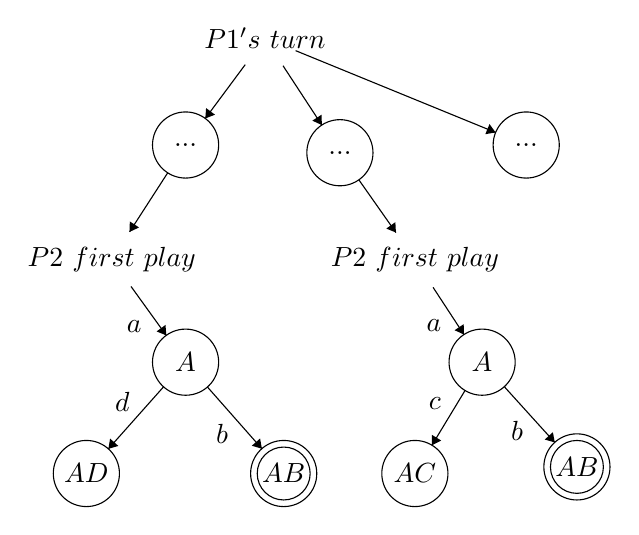
\begin{tikzpicture}[scale=0.14]
        \tikzstyle{every node}+=[inner sep=0pt]
        %\draw [black] (34.6,-5.4) circle (3);
        \draw (34.6,-5.4) node {$P1's\mbox{ }turn$};
        \draw [black] (27.4,-15.1) circle (3);
        \draw (27.4,-15.1) node {$...$};
        \draw [black] (27.4,-34.8) circle (3);
        \draw (27.4,-34.8) node {$A$};
        \draw [black] (41.4,-15.8) circle (3);
        \draw (41.4,-15.8) node {$...$};
        %\draw [black] (20.7,-25.5) circle (3);
        \draw (20.7,-25.5) node {$P2\mbox{ }first\mbox{ }play$};
        %\draw [black] (48.2,-25.5) circle (3);
        \draw (48.2,-25.5) node {$P2\mbox{ }first\mbox{ }play$};
        \draw [black] (54.3,-34.8) circle (3);
        \draw (54.3,-34.8) node {$A$};
        \draw [black] (36.3,-44.9) circle (3);
        \draw (36.3,-44.9) node {$AB$};
        \draw [black] (36.3,-44.9) circle (2.4);
        \draw [black] (62.9,-44.3) circle (3);
        \draw (62.9,-44.3) node {$AB$};
        \draw [black] (62.9,-44.3) circle (2.4);
        \draw [black] (48.2,-44.9) circle (3);
        \draw (48.2,-44.9) node {$AC$};
        \draw [black] (18.4,-44.9) circle (3);
        \draw (18.4,-44.9) node {$AD$};
        \draw [black] (58.3,-15.1) circle (3);
        \draw (58.3,-15.1) node {$...$};
        \draw [black] (32.81,-7.81) -- (29.19,-12.69);
        \fill [black] (29.19,-12.69) -- (30.07,-12.35) -- (29.26,-11.75);
        \draw [black] (25.78,-17.62) -- (22.32,-22.98);
        \fill [black] (22.32,-22.98) -- (23.18,-22.58) -- (22.34,-22.03);
        \draw [black] (22.45,-27.93) -- (25.65,-32.37);
        \fill [black] (25.65,-32.37) -- (25.58,-31.42) -- (24.77,-32.01);
        \draw (23.46,-31.53) node [left] {$a$};
        \draw [black] (36.24,-7.91) -- (39.76,-13.29);
        \fill [black] (39.76,-13.29) -- (39.74,-12.35) -- (38.9,-12.89);
        \draw [black] (43.12,-18.26) -- (46.48,-23.04);
        \fill [black] (46.48,-23.04) -- (46.43,-22.1) -- (45.61,-22.68);
        \draw [black] (49.85,-28.01) -- (52.65,-32.29);
        \fill [black] (52.65,-32.29) -- (52.63,-31.35) -- (51.8,-31.9);
        \draw (50.64,-31.47) node [left] {$a$};
        \draw [black] (29.38,-37.05) -- (34.32,-42.65);
        \fill [black] (34.32,-42.65) -- (34.16,-41.72) -- (33.41,-42.38);
        \draw (31.31,-41.3) node [left] {$b$};
        \draw [black] (56.31,-37.02) -- (60.89,-42.08);
        \fill [black] (60.89,-42.08) -- (60.72,-41.15) -- (59.98,-41.82);
        \draw (58.06,-41.01) node [left] {$b$};
        \draw [black] (52.75,-37.37) -- (49.75,-42.33);
        \fill [black] (49.75,-42.33) -- (50.59,-41.91) -- (49.74,-41.39);
        \draw (50.61,-38.58) node [left] {$c$};
        \draw [black] (25.4,-37.04) -- (20.4,-42.66);
        \fill [black] (20.4,-42.66) -- (21.3,-42.4) -- (20.55,-41.73);
        \draw (22.36,-38.39) node [left] {$d$};
        \draw [black] (37.38,-6.54) -- (55.52,-13.96);
        \fill [black] (55.52,-13.96) -- (54.97,-13.2) -- (54.59,-14.12);
        \end{tikzpicture}
}
~ %add desired spacing between images, e. g. ~, \quad, \qquad, \hfill etc.
  %(or a blank line to force the subfigure onto a new line)
  \subcaptionbox{The EPIC-gamegraph corresponding to the gametree in (a). The two nodes labeled $AB$ are merged as well as the states labeled $A$ and the state where Player 2 can play first.\label{fig:epicgg}}%
[.48\linewidth]{
  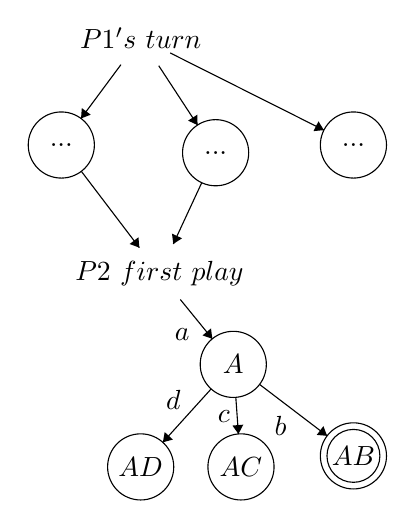
\begin{tikzpicture}[scale=0.14]
    \tikzstyle{every node}+=[inner sep=0pt]
    %\draw [black] (34.6,-5.4) circle (3);
    \draw (34.6,-5.4) node {$P1's\mbox{ }turn$};
    \draw [black] (27.4,-15.1) circle (3);
    \draw (27.4,-15.1) node {$...$};
    \draw [black] (41.4,-15.8) circle (3);
    \draw (41.4,-15.8) node {$...$};
    %\draw [black] (36.3,-26.8) circle (3);
    \draw (36.3,-26.8) node {$P2\mbox{ }first\mbox{ }play$};
    \draw [black] (43,-35) circle (3);
    \draw (43,-35) node {$A$};
    \draw [black] (53.9,-43.3) circle (3);
    \draw (53.9,-43.3) node {$AB$};
    \draw [black] (53.9,-43.3) circle (2.4);
    \draw [black] (43.7,-44.3) circle (3);
    \draw (43.7,-44.3) node {$AC$};
    \draw [black] (34.6,-44.3) circle (3);
    \draw (34.6,-44.3) node {$AD$};
    \draw [black] (53.9,-15.1) circle (3);
    \draw (53.9,-15.1) node {$...$};
    \draw [black] (32.81,-7.81) -- (29.19,-12.69);
    \fill [black] (29.19,-12.69) -- (30.07,-12.35) -- (29.26,-11.75);
    \draw [black] (36.24,-7.91) -- (39.76,-13.29);
    \fill [black] (39.76,-13.29) -- (39.74,-12.35) -- (38.9,-12.89);
    \draw [black] (40.14,-18.52) -- (37.56,-24.08);
    \fill [black] (37.56,-24.08) -- (38.35,-23.56) -- (37.44,-23.14);
    \draw [black] (38.2,-29.12) -- (41.1,-32.68);
    \fill [black] (41.1,-32.68) -- (40.98,-31.74) -- (40.21,-32.37);
    \draw (39.09,-32.33) node [left] {$a$};
    \draw [black] (45.39,-36.82) -- (51.51,-41.48);
    \fill [black] (51.51,-41.48) -- (51.18,-40.6) -- (50.57,-41.4);
    \draw (47.3,-39.65) node [below] {$b$};
    \draw [black] (43.23,-37.99) -- (43.47,-41.31);
    \fill [black] (43.47,-41.31) -- (43.91,-40.47) -- (42.92,-40.55);
    \draw (42.74,-39.7) node [left] {$c$};
    \draw [black] (37.28,-6.75) -- (51.22,-13.75);
    \fill [black] (51.22,-13.75) -- (50.73,-12.95) -- (50.28,-13.84);
    \draw [black] (29.22,-17.49) -- (34.48,-24.41);
    \fill [black] (34.48,-24.41) -- (34.4,-23.47) -- (33.6,-24.08);
    \draw [black] (40.99,-37.23) -- (36.61,-42.07);
    \fill [black] (36.61,-42.07) -- (37.52,-41.82) -- (36.78,-41.14);
    \draw (38.26,-38.19) node [left] {$d$};
    \end{tikzpicture}
    }
  \caption[Epic example]{EPIC example}
  \label{fig:epicex}

\end{center}

\end{figure}

EPIC is an enhancement proposed by \cite{whitehouse14} and aims to take advantage of the episodic nature of certain games. The idea is that instead of discovering the same strategy for very similar situations (episodes) in different parts of the game tree, EPIC puts them together such that those similar situations are the same and thus only have to be discovered once. \newline
It yielded good improvements in \textit{Dou Di Zhu} and it stands to reason that it does also help in Tichu.
\textit{Dou Di Zhu} has the same trick system as Tichu, but it is played with only 3 players and the playable combinations are slightly different. But overall the two games are similar very to each other.

In \textit{Dou Di Zhu} and Tichu, an episode is naturally defined by a trick (from first play until all players pass consecutively). The \textit{position in episode} of a node is the path from the node upwards until the beginning of the trick is reached. An example is shown in Fig.~\ref{fig:piepic}.
Similar on how all nodes belonging to the same \textit{information set} were put together for ISMCTS, for EPIC, all states with the same \textit{position in epic} are merged into one node creating an EPIC-gamegraph. The result for the example is shown in Fig.~\ref{fig:epicgg}.
For Tichu, the gamegraph contains 4 "root nodes" corresponding to the 4 states where a particular player can play first.

The search is then performed on this gamegraph according to ISMCTS. To implement EPIC very little change to ISMCT is required. Only the way how gamestates are mapped to nodes has to be modified. The rest of the algorithm is identical.

EPIC reduces the branching factor dramatically since many different nodes are merged. The ordering of different tricks in the game is basically removed, which, of course, introduces some new difficulties and is probably the main reason why it did not perform well on Tichu.

\subsubsection{Move groups}
Another way to reduce the branching factor and possibly improve UCT decisions are \textit{move-groups}.
The idea is to divide the actions into (not necessarily disjoint) groups. Those groups are then inserted as an additional layer after each node in the gametree.
The decision in the \textit{tree policy} then becomes a two-step process. First select a group and then an action belonging to that group (UCT can be used in both phases).
Move groups are introduced in \cite{movegroups} and further examined in \cite{movegroups2}.

This enhancement reduces the effective branching factor and has been shown to help with move selection when similar valued moves appear. However, it is not trivial to find good groups. \cite{movegroups2} found that random groups did neither improve nor worsen the simulation efficiency, but increased the speed. Grouping the best nodes together seems to yield the best result, but finding the best nodes is exactly the problem.

I decided on putting all actions of the same \textit{combination-type} into the same group. With the idea that they most of the time lead to similar results and thus the chance that the best actions are in the same group are increased.
% TODO NOTE: maybe hight/rank and "probability" are better groups.

Surprisingly, ISMCTS with \textit{move-gropus} performed very poorly against the default ISMCTS agent (more in section \ref{sec:movegroupsexp}).


\subsection{Determinization}
\label{sec:determinization}
\textit{Whitehouse} shows in \cite[p.~54+]{whitehouse14} that for the game \textit{Dou Di Zhu}, more than 20 determinizations per search yield diminishing returns, and the more simulations per determinization are made, the better the agent plays.
Assuming this is value is similar in Tichu I decided to generate 30 different determinizations per search, just to be on the save side (Tichu has one player more).

The problem of creating determinizations in Tichu boils down to infer the remaining handcards of the other players. Even for human players this is hard and involves a lot of guesswork and knowledge about the game and the other player. However, it turns out that the extend of the advantage of good determinizations it is not exactly clear. For more see section~\ref{sec:cheatexp} and \cite{ismcts}.

To avoid using \textit{domain knowledge}, I decided to use data of existing human games. \textit{Brettspielwelt.de} is an online platform that provides the possibility to play different games online against other other players. One to the offered games is Tichu. The game-logs of played Tichu games can be found at \textit{log.tichumania.de} \cite{tichumania}, where about 500'000 games of 5'000 different players are stored.
Sadly, the \textit{Brettspielwelt} team did not respond to my inquiry for the entire dataset displayed there, and I had to write a scraper to obtain the gamelogs.
In the following sections the obtained data is visualized and different strategies to exploit the pattern in the data are discussed.

\subsubsection{Random}
The easiest determinization strategy is to distribute the unknown cards uniformly at random amongst the other players.
Note that the observer player knows his own handcards and which cards already have been played. Therefore it can deduce exactly which cards are among the handcards of the other players, as well as how many cards each player has.


\subsubsection{The Data}
The goal is to determine the prior probability of a given set of cards of size $n$ (a player has $n$ handcards) to contain a particular combination. That is, the answer to the question: "what is the probability that a player, having 6 cards left, possesses a pair of kings"?

First I have to introduce the notion of a \textbf{General Combination}. A "normal" combination is a set of cards, each with its rank and suit. A \textit{General Combination} however is suit agnostic. So the combinations ($K\heartsuit, K\diamondsuit$) and ($K\diamondsuit, K\clubsuit$) are two distinct combinations, but belong to the same \textit{General Combination}, which is $Pair(King, 1)$ \newline
More formal: A \textit{General Combination} is the triple (\textit{combination-type}, \textit{height}, \textit{length}), where \textit{combination-type} is one of [Single, Pair, Triple, Square, Fullhouse, Straight, Pairstep, SquareBomb, StraightBomb], \textit{height} is the value of the combination and \textit{length} denotes how many cards belong to the combination (this is used to distinguish straights and pairsteps).

There are 255 different \textit{general combinations}, about 100 of them are extremely rare (a straight of length 14 practically never appears for example).

To approximate the probability for each of those \textit{general combinations} appearing in different sized handcards, I scraped around 2 million different handcards sets\footnote{In a game, each time a player plays some combination, the remaining handcards are stored (as well as the initial cards at the beginning of the game.)} from the \textit{tichumania} website and counted which \textit{general combinations} appear how many times. In total there are about 12 million \textit{general combinations} in those 2 million handcards, giving an average of about 6 different \textit{general combinations} per hand.
Some of the results are shown in Fig.~\ref{fig:hc}, the remaining plots can be found in the appendix~\ref{hc_appendix}.

Figure~\ref{fig:hc1} shows the distribution  when a player has only one single card left. With one card, only the \textit{Single combination-type} is possible.\newline
It is clearly visible that the player is more likely to have either a low card (2, 3 or 4) or a high card (King, Ace) than to have a 7 or 8.
The special cards have an overall lower probability of occurring because there is only one of each and not four. Nevertheless, The Mahjong almost never is the last card\footnote{It is customary (and smart) to play the Mah-Jong in the first trick, which explains the low probability.}, while the Dog is almost as likely to appear as a 7.
It makes sense that either low or high cards "survive" longer than medium ranked cards. High cards are advantageous at the end of the game because it is easier to finish with them, so players take care to keep them, where as low cards are harder to get rid of, and therefore they persist until the end. Another reason why low cards are that common, is that an often seen strategy is to play one high card as second last to win the trick and then to play the low card to finish. The high probabilities for high cards in Figure~\ref{fig:hc2} confirms this.

Figure~\ref{fig:hc2} shows the probabilities for 2 remaining handcards. It is very likely that at least one of the two cards is an Ace, followed by the King and Queen. Interestingly, the dragon and phoenix are also rather likely.
With 2 cards, it is possible to have a pair, however they seem to be distributed uniformly and only very small trends can be inferred (for example an Ace-pair is lower, while the 2-pair is slightly higher than all others).

Skipping some steps, figure~\ref{fig:hc5} shows the probabilities for 5 remaining handcards. The single cards are still clearly distributed, and also the pairs seem to diverge from a uniform distribution. All other combinations however are too infrequent to have a clear distribution.

Figure~\ref{fig:hc12} shows the distribution for 12 cards and it is clear, the more cards, the closer to uniform each combination distribution gets. This makes sense since in the beginning (with 14 cards) they should be uniformly distributed due to the random deals.

This analysis shows that especially towards the end of the game, this prior data can help to create better (more accurate) determinizations compared to the random determinization.

In the next two sections, two strategies to create determinizations using this data are described.

\begin{figure}[hb]
    \begin{center}
        \begin{subfigure}[h]{.8\textwidth}\includegraphics[width=\textwidth]{images/det/type_for_len_1}
            \caption{1 card: Only singles are possible with one card left. Low and high cards are more likely to appear than middle ranked cards. The Mah-Jong is seldom the last card, but the Dog appears more often than expected.}
            \label{fig:hc1}
        \end{subfigure}

        \begin{subfigure}[h]{.8\textwidth}\includegraphics[width=\textwidth]{images/det/type_for_len_2}
            \caption{2 cards: Single cards are similar but not the same as in (a). Higher cards are more now more likely than lower cards. Pairs might appear, but there is no apparent significant trend.}
            \label{fig:hc2}
        \end{subfigure}
    \end{center}
\end{figure}~\begin{figure}[ht]\ContinuedFloat
    \begin{center}
        \begin{subfigure}[h]{.8\textwidth}\includegraphics[width=\textwidth]{images/det/type_for_len_5}
            \caption{5 cards: Single cards are very similar to (b), and high Pairs are slightly more likely than lower ones. All other combinations seem to be distributed uniformly at random.}
            \label{fig:hc5}
        \end{subfigure}
        \begin{subfigure}[h]{.8\textwidth}\includegraphics[width=\textwidth]{images/det/type_for_len_12}
            \caption{12 cards: No obvious trend is visible. This is not surprising as only 2 cards have been plaid.}
            \label{fig:hc12}
        \end{subfigure}
    \end{center}
\caption[Determinization Handcards Plot]{The Plots for the Handcard Data}
\label{fig:hc}

\end{figure}

\subsubsection{Combination Determinization}
This strategy selects entire combinations and gives them to the player which is most likely to have it.

First, all possible combinations that might appear in any of the handcards of the players are generated. For each of those combinations three probabilities are calculated and summed together (one for appearing in each players handcards). Each possible combination thus has a score approximately proportional to the probability of actually appearing in any of the handcards. Then combinations are repeatedly sampled (weighted by their score) and "given" to the player most likely to have them, until all cards are distributed.
There is of course some bookkeeping to make sure all players get the right amount of cards and that no card is lost or created during the process. But this is an implementation detail.

The problem with this strategy is that combinations that are very unlikely are selected too often because the differences between the probabilities are not especially high. And indeed, the experiments show that it is even worse than the random determinization (section~\ref{sec:detexp}).


\subsubsection{Single Determinization}
The data shows that single cards are the only \textit{combination-type} other than the pair, which is not distributed uniformly at random.
This strategy aims to exploit that. Instead of generating all possible combinations, it looks at each player in ascending order of their number of handcards and gives them one card at the time, sampled from the remaining cards.\newline
So players with less cards left, get their cards first and the determinization is more likely to "hit" correct cards for them. From experience it is more important to know the enemies cards when they have only a few left, since I want to prevent them from finishing.

In the experiments, this strategy performed at least as well as the random determinization (section~\ref{sec:detexp}).


\subsubsection{Machine Learning approach}
I tried to train 14 different models (one for each size of handcards $N$). Given all the unknown cards and all cards already played by a player, the model should predict which $N$ cards the player has in his hands.
The idea being that the history of actions and the remaining cards are correlated. Together with the possible cards, it might be possible to predict something.
However, I did not manage to create a model that converges. The data is probably too noisy and too sparse to infer anything. In addition, "near misses" are also counted as wrong. The evaluation should have a concept of "closeness" of the cards. For example giving a 10 instead of a 9 is much better than giving a King. The models often get one or two cards right, but that is not better than random.\newline
Sadly there was no more time left to explore more in this direction.


\subsection{Rollout}
\label{sec:rollout}
As a reminder: The rollout phase simulates a game from a given gamestate to a terminal one, following a (fast) action selection strategy (\textit{default policy}). The goal is to estimate an initial value for the given gamestate.

The rollout phase is an important part for the overall playing strength of the agent. The closer the \textit{default policy} imitates the strategy of the enemy, the better the initial estimation of each gamestate gets, and with it the \textit{tree policy} can pick the next action more accurately, which in turn yield an better final decision. \newline
Funnily enough, this implies that the best \textit{default policy} when playing against the \textit{random} agent, a random \textit{default policy} would be the best.


\subsubsection{Random Rollout}
The random rollout \textit{default policy} selects one action uniformly at random out of all legal actions.
It is very fast and enables many rollouts to be performed. However, it suffers from multiple problems. One of which (in my opinion the most problematic) is that it, in some sense, only approximates the number of paths that lead to a win (or loss). It does not account for "obviously good/bad moves" being played more or less often and thus simulates games that will never happen, resulting in quite random rewards.\newline
Despite this, it still works because in most cases, good states more often than not lead to a win, and bad states have more paths to a loss.

In the endgame of Tichu, when a big part of the gametree can be explored during a search, a random \textit{default policy} might even be sufficient. Especially when only 2 players remain, there is no hidden information anymore (all cards can be inferred) and a rollout is quickly done (the end of the game is near).

\subsubsection{Last Good Response With Forgetting (LGRF)}
\label{sec:lgrf}
LGRF aims to be an enhancement to the random \textit{default policy}. Actions are still selected uniformly at random, with one exception: When a previous stored action is encountered, the response to that action is always selected.
During a rollout, all pairs of actions are recorded as  \textit{(action$\rightarrow$ response)}-tuples. After the rollout, the responses of the players that won are stored and the responses of the players that lost are deleted (forgotten) from the storage.\cite{whitehouse14}\newline

The idea is to keep the good actions, and forget the bad ones. This works good for games where the same action always has a similar 'value' independent of the circumstances or actions often depend on the previous one. Tichu does not exactly fulfill this criteria. Many \textit{(action$\rightarrow$ response)}-tuples make sense, for example, "play single 2 $\rightarrow$ play single 3" is a perfectly good reaction. However, for a player to win he plays a \textit{King} on a $2$. Then the "play single 2 $\rightarrow$ play single \textit{King}" is stored, and in the next rollout the player always plays a \textit{King} on a $2$, which is probably bad.

Then there is the problem with the \textit{pass} action. It is by far the most used action and seldom played as a response on another action. Furthermore, combinations are played on other combinations, independent of whether a player passed in between or not. Thus pass actions are ignored with respect to LGRF.

Sadly, but not surprisingly, LGRF decreased the playing strength of an agent compared to a purely random rollout.

\subsubsection{No Rollout}
There is the possibility of doing no rollout at all. That is, all actions are added to the gametree and chosen according to UCT. Note that this still mostly ends up in randomly selecting actions since UCT selects randomly among, as of yet, unvisited nodes. However, it makes sense together with EPIC. Since the EPIC-gamegraph contains loops, the algorithm will reach nodes that are already (at least) partially explored and there the additional UCT information might improve the search.

\subsubsection{Neural network Rollout}
\textit{AlphaGo} uses MCTS, with a deep neural network (NN), trained on human expert games, as \textit{default policy} \cite{alphago}. They use another NN as \textit{tree policy}, which is trained by self-play with reinforcement learning methods.
So I thought whether it is possible to train a NN for Tichu and use it as \textit{default policy}. See section~\ref{sec:nn_agents} for the description of the agents.


\section{Neural Network Agents}
\label{sec:nn_agents}
As an enhancement to the MCTS agents, several Deep-Q-learning (DQN) agents were implemented.
The agents only differ in the network architecture. To train the network, the Deep-Q-learning algorithm implemented in the Keras-rl package\cite{kerasrl} was used.

The goal was to use the neural network agents as the \textit{default policy} in the MCTS agent.


\subsection{Architectures}
The input to the network consists of the handcards of all players, the combination on the table and some information about the current ranking.
I tested two different 'encodings' for a set of cards:
\begin{enumerate}
    \item Boolean Vector of length 56: Each card has a different number ranging from 0 to 55. If a card with number $n$ is contained in the set, then the bit at position $n$ in the vector is set to $1$ (or $True$).
    \item Integer Vector of length 17: Each rank has a different number ranging from 0 to 16. This includes special cards (Dog=0, Mahjong=1, Two=2, ..., King=13, Ace=14, Dragon=15, Phoenix=16). The vector then represents how many cards of each rank appear in the set.
\end{enumerate}

Both representations have their advantages and disadvantages. 1) leads to a rather long but boolean input, while 2) discards information about the suits of the card in favor to a shorter, but numeric representation.

I tested two different architectures. Both have 2 hidden, fully connected layers, with 'elu'\footnote{see https://en.wikipedia.org/wiki/Activation\_function}  as activation function.
\begin{enumerate}
    \item Together: Connects the input vector directly to the 2 hidden layers.
    \item Separate: Takes the input vector and splits it into the 6 separate components (4 players handcards, the combination on the table and the ranking-information). Each component then connects to a 'private' hidden layer before concatenating them to the second 'shared' hidden layer.
\end{enumerate}

The output layer has 258 neurons, which corresponds to the number of possible actions at any time in the game.

A visualization of the architecture can be found in Fig.~\ref{fig:nnarchi}

A particular challenge was to make sure the agent plays only legal moves. This was solved by adding a last layer which subtracts $500$ from the output neurons representing a illegal action. The Q-values (output neurons) of illegal actions are thus lower than the others, and the agent chooses an legal action. To do so, a vector encoding the legal actions had to be given as another input to the network.

The essential information about the current ranking of the players is encoded in 2 bits. The first bit indicates whether the teammate finished first, the second bit whether an enemy finished first. Note that at most one of the two bits is set to 1 since only one player can finish first. In the \textit{Together} architecture, the bits are contained in the input vector, while in the \textit{Separate} architecture they also are a separate input.



\begin{figure}[hb]
    \begin{center}
        \begin{subfigure}[h]{.8\textwidth}\includegraphics[width=\textwidth]{images/nnarchi_together}
            \caption{Together NN architecture. Layer 1) has the same number of neurons as the input vector and is fully connected to the second layer which has 258 neurons. The \textit{legal Actions input} reduces the q-values of the illegal actions by 500 in order to prevent the agent from selecting them. }
            \label{fig:archi1}
        \end{subfigure}

        \begin{subfigure}[h]{.8\textwidth}\includegraphics[width=\textwidth]{images/nnarchi_seperate}
            \caption{Separate NN architecture. Each input is fully connected to a "private" set of neurons (1). Those neurons are then concatenated to a single layer which is in turn fully connected to the second hidden layer (2) of length 258.\textit{legal Actions input} is the same as in (a). }
            \label{fig:archiw}
        \end{subfigure}
    \end{center}
\caption[Neural Network Architectures]{The two Neural Network Architectures.}
\label{fig:nnarchi}

\end{figure}

\subsection{Training}
To train the network, the Deep-Q-learning algorithm implemented in the \textit{Keras-rl} library\cite{kerasrl} was used.

As training policy for the DQN-agent I used the Bolzman-policy with linearly decreasing $\tau$.
With the Bolzman-policy, each action $a$ has following  probability of being selected:

$$
p(q_a) = \frac{\exp(\frac{q_a}{\tau})}{\sum_{k \in Actions} \exp(\frac{q_k}{\tau})}
$$
where $q_a$ denotes the value of the output neuron corresponding to action $a$ (the q-value of $a$).
$\tau$ determines the exploration/exploitation ratio. The higher $\tau$, the more exploration is done.\newline
This function selects the highest q-value with very high probability when $\tau$ is small (exploitation). However, when $\tau$ is big, all actions have the same probability of being selected (exploration).

During training, the agent plays multiple games with three other agents. Those other agents are either 3 random agents, 3 other (already trained) DQN agents or 3 MCTS agents.
Each agent is trained for 1 million steps, which corresponds approximately to 300'000 games.

Some trainings are visualized in Fig.~\ref{fig:nntrain}

\begin{figure}[hb]
    \begin{center}
        \begin{subfigure}[h]{.5\textwidth}\includegraphics[width=\textwidth]{images/DQNAgent2L_56x5_2_sep_random_2017-06-05_15-25-01_steps_1000000}
            \caption{DQN with the \textit{Seperate} Architecture and the 56-boolean input, trained for 1 million steps against 3 random agents. There is no real improvement during the training. The mean-q values approximate the episode reward somewhat.}
        \end{subfigure}
\\
        \begin{subfigure}[h]{.4\textwidth}\includegraphics[width=\textwidth]{images/DQNAgent2L_56x5_2_sep_learning_2017-05-27_20-01-57_steps_1000000_tau}
            \caption{The same agent as in (a) but trained against itself. No improvement can be seen in the episode reward, but the q-values increase when $\tau$ reaches 0.2.}
        \end{subfigure}~
        \begin{subfigure}[h]{.48\textwidth}\includegraphics[width=\textwidth]{images/DQNAgent2L_56x5_2_sep_learning_2017-06-06_17-12-32_steps_1000000}
            \caption{A second training period for the agent in (b), but with a constant $\tau$ of 0.2. All values converge really quickly and no change happens afterwards. }
        \end{subfigure}
    \end{center}
\caption[Neural Network Training]{Two trainings on different environments. b) and c) are two training periods of the same agent.}
\label{fig:nntrain}

\end{figure}
